\chapter{Research design}\label{chap:research}

The research design section outlines the procedures to accomplish the objectives and enhance the understanding of the subject matter. It presents the methodology as a series of interconnected steps, each crucial for tackling research questions and achieving goals. The following sections further elaborate on these steps and their significance to the research.


\section{Simulate Thread Networks using OTNS and Codelab with Docker}\label{sec:simulation}
The research used OpenThread Network Simulator (OTNS) and Codelab with Docker to simulate Thread networks under different conditions. OTNS is a powerful tool for creating, visualizing, and analyzing virtual Thread networks, while Codelab offers hands-on tutorials for simulating Thread networks in a Docker container environment. This setup allowed accurate emulation of real-world Thread network behavior and efficient execution of numerous simulations. The combination of these tools facilitated a deeper understanding of Thread network principles and mechanisms, enabling the analysis of various configurations and their impact on performance metrics like latency, throughput, and energy consumption, thus paving the way for a more informed optimization process.

\section{Mathematical Constraints for Building a Thread Network}\label{sec:mathematical_constraints}
The objective of the mathematical model is to build a Thread network that adheres to specific mathematical constraints, ensuring a well-functioning network with the required device types, sensitivity, and received signal strength intensity (RSSI). The following mathematical model is designed for this purpose:

\begin{equation}\label{eq:minimize_power}
    \begin{aligned}
        Min\sum_{i=1}^{M}P_t^i
    \end{aligned}
\end{equation}

    \textbf{Subjects to:}
\begin{equation}\label{eq:mathematical_constraints_end_device}
    \begin{split}
        RSSI_{ED}^j>EDSensitivity,j\in1,\cdots,N \\
        -20dbBm{\le P}_t^j\le8dBm \\
        N_{REED}=n_{Router}+n_{Leader} \\
    \end{split}
\end{equation}

\begin{equation}\label{eq:mathematical_constraints_router}
    \begin{split}
        {RSSI}_{Router}^k>RouterSensitivity,k\in1,\cdots,O \\
        -{20dBm\le P}_t^k\le8dBm
    \end{split}
\end{equation}

\begin{equation}\label{eq:mathematical_constraints_border_router}
    \begin{split}
        {RSSI}_{BD}^L>BDSensitivity,L\in1,\cdots,P \\
        -{20dBm\le P}_t^L\le8dBm \\
        Sensitivity=-100dBm \\
        SEED\in0,1 \\
        n_{Leader}=1 \\
        n_{Router}+n_{Leader}\geq3 \\
        n_{BR}=2
    \end{split}
\end{equation}

    Where $P_t$ represents the Transmit Power of each one of the $M$ devices, $RSSI$ is the Received Signal Strength Intensity, $ED$ is End Device, $REED$ is Router Eligible End Devices, $N_{REED}$ is the number of the REEDs, $n_{Router}$ is the number of the routers, $n_{Leader}$ is number of the leaders, $N$ is amount of end devices, $O$ is the number of Routers, $P$ is the number of Border Routers, $SEED$ is Sleepy End Devices, and $Sensitivity$ is $-100 dBm$ with IEEE 802.15.4 \cite{Semiconductor_Nordic_Product_Brief_2018_2.0}.

\vspace{2mm}
The model seeks to minimize the transmitted power of each device while ensuring adequate signal strength, proper device type distribution, and network resilience. By complying with these constraints, the Thread network can be effectively optimized for both performance and energy consumption.

The constraints of the model are as follows:

\vspace{2mm}
\begin{itemize}
    \item To establish a link between the sensors and the End Devices (EDs), the Received Signal Strength Intensity (RSSI) of each ED must be approximately above the sensitivity of each ED. This ensures a stable connection between the devices.
    \item The maximum transmission power of each End Device is limited to $8 dBm$ to minimize energy consumption while maintaining effective communication.
    \item The number of Router Eligible End Devices (REEDs) must be equal to the number of Routers + the Leader because, if a Router is lost, a connected REED must become a Router to replace the "Dead Router" and maintain network resilience.
    \item To establish a connection between the EDs and routers, the RSSI of each Router must be approximately above the Sensitivity of each Router. This guarantees a stable link between the devices and the Routers.
    \item The maximum transmission power of each Router is also limited to $8 dBm$, conserving energy while maintaining efficient communication.
    \item To establish a connection between the Routers and Border Routers, the RSSI of each Border Router must be approximately above the sensitivity of each Border Router, ensuring a reliable link between the network components.
    \item The maximum transmission power of each Border Router is also set to $8 dBm$, optimizing energy consumption while maintaining effective communication within the network.
\end{itemize}
\vspace{3mm}


\section{Monte Carlo Method for Initial Buildup}\label{sec:monte_carlo_method}
Monte Carlo Method is utilized to build the initial Thread network, considering various factors such as the distance between devices, the total number of devices, device types, device positions, and transmission power. The Monte Carlo method comprises several steps, each with its distinct processes.

These steps are separated and explained in detail as follows:

\subsection{Step 1: Start}\label{sec:monte_carlo_method_step_1}
The Monte Carlo method is initiated to optimize the Thread network, considering the key parameters influencing the network's performance and energy efficiency.

These parameters are outlined in the table below:

\begin{longtblr}[
  caption = {Parameters influencing Monte Carlo Method.},
  label = {tab:mcm_parameters},
  ]{
  colspec = {X[5cm] X[10cm]},
  hlines, vlines,
  rowhead = 1, % Repeat the header row on every page
  row{1} = {font=\bfseries},
}
  Parameter & Description \\
  Distance & The distance between the devices \\
  Number of Devices & The total number of devices ($8$ for this research) \\
  Device Types & The type of each device (Unallocated, SEED, REED, Router, Leader, and Border Router) \\
  Device Positions & The position of each device, randomly generated from $1$ to $8$ \\
  Transmission Power & The transmission power of each device, randomly generated between $-20dBm$ to $8dBm$ with $4$ steps difference \\
\end{longtblr}

\subsection{Step 2: Generate Random Numbers}\label{sec:monte_carlo_method_step_2}
Based on the factors mentioned at the start, MCM generates a vector X of length equal to 2n, where n is the number of places where network elements can be allocated. Network elements include all device types and sensors.

The vector is represented as:

\begin{equation}\label{eq:vector_x}
    \begin{split}
        X=\left[x_1,x_2,x_3,\cdots x_n,p_1,p_2,p_3,\cdots,p_n\right] \\
        for{\ x}_n\in0,1,2,3,4,5 \\
        transmission\ power\ p_n\in-20:4:8\ dBm
    \end{split}
\end{equation}

    Where $0$ represents no element allocated, $1$ is allocate a SEED, $2$ is allocate a REED, $3$ is allocate a Router, $4$ is allocate the Leader, and $5$ is allocate a Border Router.
\vspace{2mm}

\subsection{Step 3: Evaluate Results}\label{sec:monte_carlo_method_step_3}
The objective function aims to build a Thread network using the minimized power value of the entire system without violating the constraints specified in the mathematical formulation. If a constraint is violated, a penalty should be added to the objective function, which is weighted according to the importance of the constraint.

The objective function with penalty values can be written as:

\begin{equation}\label{eq:objective_function}
    \begin{aligned}
        Min\sum_{i=1}^{M}P_t^i+penal_1+penal_2+penal_3\ldots+penal_{nr}
    \end{aligned}
\end{equation}

    Where $penal_1$ represents penalty for violating the first restriction, $penal_2$ is penalty for violating the second restriction, and $penal_{nr}$ is the penalty for violating the last restriction.
\vspace{2mm}

A solution is viable only if all constraints are satisfied without penalties. To ensure this, the mathematical model requirements are verified at each step. If a step fails to meet the requirements, the MCM generates new random inputs and re-evaluates the network until a constraint-compliant solution is found. This iterative process guarantees a Thread network that meets performance and energy optimization criteria.

\subsection{Step 4: End}\label{sec:monte_carlo_method_step_4}
The MCM converges on an optimal solution that satisfies necessary constraints, providing outputs such as device types, transmission power, and location. It also offers information on constraint violations, including the penalty, network power consumption, and RSSI sensitivity violations—these outputs aid in understanding the optimization process and refining the network design.


\section{Genetic Algorithm for Transmission Power Optimization}\label{sec:genetic_algorithm}
GA optimizes the Thread network's transmission power to reduce energy consumption while maintaining wireless communication quality. MCM-generated configuration is the starting point for GA.

Key steps and parameters for GA:

\begin{longtblr}[
  caption = {Parameters influencing Genetic Algorithm.},
  label = {tab:ga_parameters},
  ]{
  colspec = {X[5cm] X[10cm]},
  hlines, vlines,
  rowhead = 1, % Repeat the header row on every page
  row{1} = {font=\bfseries},
}
  Parameter & Description \\
  Population Size & The number of individuals in the population \\
  Population & The initial population consisting of transmission power, device types, and device positions \\
  Max Iteration & The maximum number of iterations \\
  Maximum Transmission Power & The minimum transmission power (dBm) \\
  Minimum Transmission Power & The maximum transmission power (dBm) \\
  Mutation Rate & The probability of mutation \\
  Selection Method & The method used for selecting individuals \\
  Mutation Method & The method used for mutating individuals \\
\end{longtblr}

In this table, the "Population" row represents the output from the Monte Carlo simulation, which is a list of transmission power, device types, and device positions.

The GA process includes the following steps:

\vspace{2mm}
\begin{enumerate}
    \item \textbf{}{Initialization:} Generate the initial population using MCM output.
    \item \textbf{}{Selection:} Choose best individuals based on fitness using the "sorted" method.
    \item \textbf{}{Crossover:} Produce offspring by crossing over selected individuals' genes.
    \item \textbf{}{Mutation:} Introduce random changes to transmission power using the "swap" method.
    \item \textbf{}{Evaluation:} Calculate fitness by assessing transmission power and RSSI penalty.
    \item \textbf{}{Termination:} Iterate until reaching the maximum number of iterations.
\end{enumerate}
\vspace{3mm}

The output is a list of optimized transmission power values for each device, along with device types, positions, and penalty values. The solution minimizes transmission power while meeting connectivity constraints.


\section{Prototype Development}\label{sec:prototype_development}
This section details the steps taken to build the prototype that applied the output from Monte Carlo and GA to validate the results. We followed the Monte Carlo output to construct the network by selecting the appropriate device types. Our setup consisted of 8 devices: 2 Border Routers, 3 Routers (with one of them automatically elected as a leader), and 3 Router Eligible Devices (REEDs). The prototype was designed to closely resemble the conceptual model presented earlier in the figure, with the only slight difference being using REEDs instead of sensors as the end devices.

An image is provided below to illustrate the Thread network topology that we have constructed.

\begin{figure}[h]
    \centering
    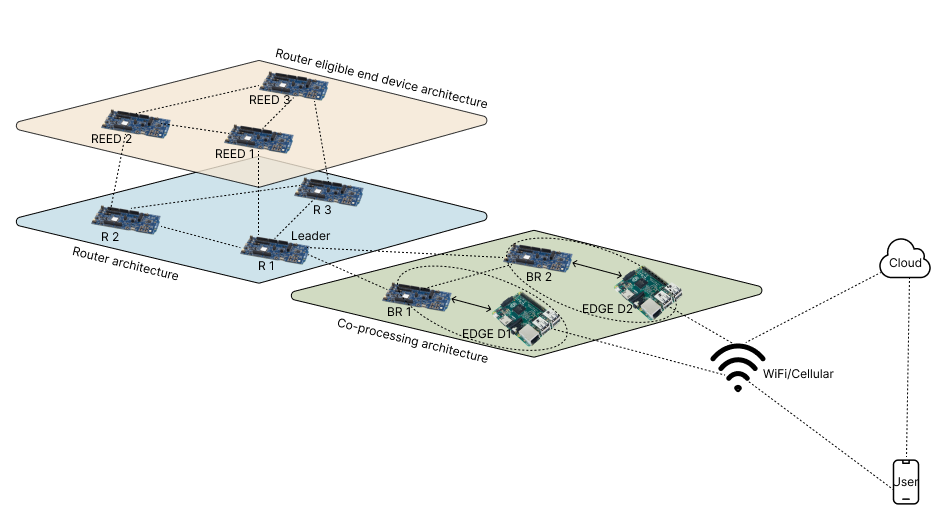
\includegraphics[width=0.8\textwidth]{images/research_design/prototype_topology.png}
    \caption{Thread network prototye topology.}
    \label{fig:prototype_topology}
\end{figure}

\subsection{Software Implementation}\label{sec:software_implementation}
The nRF-provided Thread Client and Server setup, supporting multiprotocol communication, allowed concurrent communication with Thread and BLE devices. This simplified the process of connecting non-Thread devices to the network. The setup was customized to forward data from Client nodes to the Server using CoAP, validating data transfer within the network. The setup supported both Unicast and Multicast communication out-of-the-box, making it valuable for research purposes.

\subsection{Construction Process}\label{sec:construction_process}
To construct the prototype, we followed these steps:

\vspace{2mm}
\begin{enumerate}
    \item Assigned device roles based on the output from Monte Carlo and GA, ensuring an optimal configuration for the network.
    \item Flashed each router with the Thread Server setup and each REED with the Thread Client setup. In this configuration, routers acted as servers, while REEDs acted as clients. Communication between devices was bidirectional, with the clients having BLE enabled for multiprotocol support.
    \item Flashed the Border Router nodes with the Coprocessor setup provided by nRF. To enable the Raspberry Pi to act as an Edge device, we implemented the OpenThread Radio Coprocessor (RCP) architecture.
    \item Turned on the devices one by one, noting that the first device activated in the network is most likely to become the leader, although leadership can change during the network's lifetime.
    \item Validated all the nodes by running multicast messages using Thread ICMP service. The ICMP service allowed us to send echo requests (ping) to devices, activating their Thread antennas. This allowed us to test the Thread connection, and devices could also reply.
    \item Validated the multiprotocol support connection by running a data flow from the ESP32 UWB devices to the REEDs, which then forwarded the data to the routers. This step ensured seamless communication between non-Thread devices and the Thread network.
    \item Monitored the network for stability and performance, adjusting settings to maintain optimal operation.
\end{enumerate}
\vspace{3mm}

Following these steps, we successfully constructed the prototype to apply the optimized settings obtained from the Monte Carlo simulation and the Genetic Algorithm. The following figure presents a real-world Thread network prototype setup. The image provides a clear view of the nRF52840-based Thread nodes, Raspberry Pi as the Edge device, and the Border Router setup with the Dongle. It also showcases the Development Kits used for Routers and REEDs.

\begin{figure}[h]
    \centering
    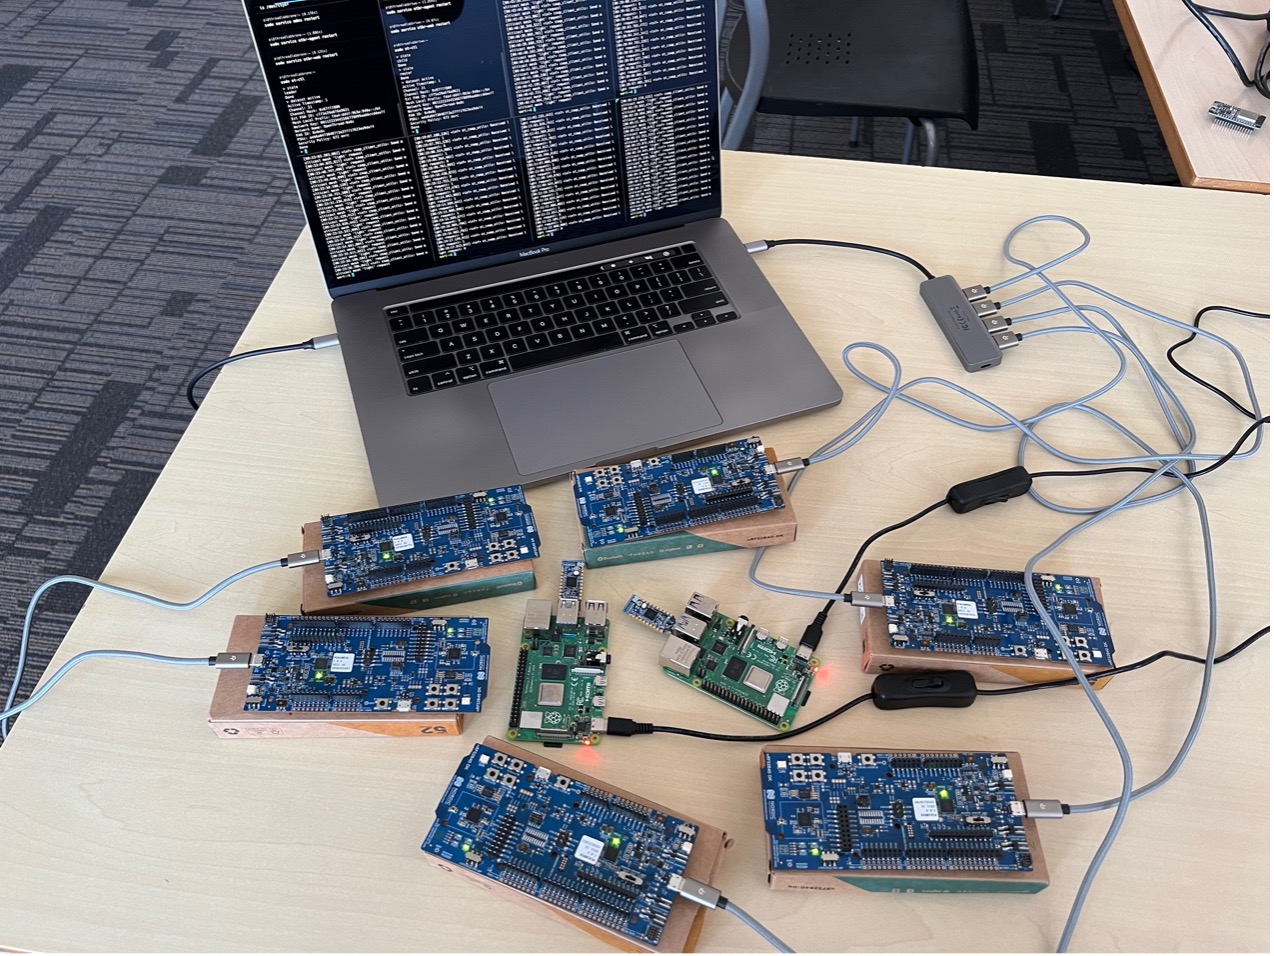
\includegraphics[width=0.6\textwidth]{images/research_design/prototype_setup.jpg}
    \caption{Thread network prototype setup in the lab.}
    \label{fig:prototype_setup}
\end{figure}

In the next section, we will discuss the multiprotocol support in more detail, addressing the connection of non-Thread devices with the Thread network.


\subsection{Multiprotocol Support}\label{sec:multiprotocol_support}
The nRF52840 hardware’s multiprotocol support, enabled by the MPSL library, allows integration of non-Thread devices like ESP32 UWB devices. MPSL provides services for multiprotocol apps and facilitates transmission timeslot negotiation. SoftDevice Controller ensures MPSL support as a Bluetooth LE Controller implementation. The dynamic solution enables the simultaneous operation of multiple radio protocols, requiring only radio peripheral reinitialization when switching between protocols \cite{nordic_multiprotocol_support}.

\begin{figure}[h]
    \centering
    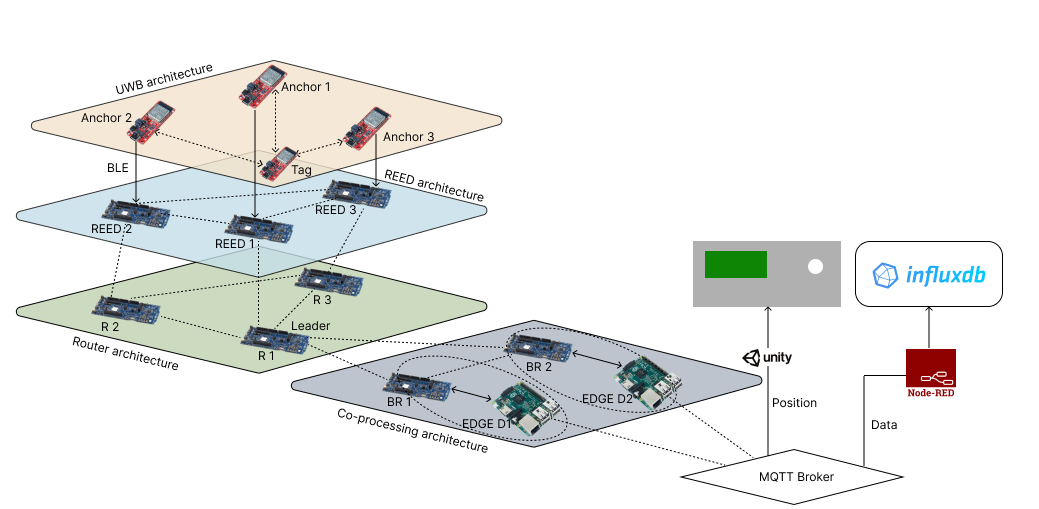
\includegraphics[width=0.8\textwidth]{images/research_design/multiprotocol_support.png}
    \caption{Multiprotocol support architecture.}
    \label{fig:multiprotocol_support}
\end{figure}

Figure \ref{fig:multiprotocol_support} shows ESP32 UWB devices connected via BLE to the Thread network, enabled by nRF52840 SoC's multiprotocol support. ESP32 UWB devices bridge non-Thread devices and the Thread network, connecting to REEDs via BLE. This integration highlights network adaptability to various devices. Multiprotocol support expands the device range that can interact with the Thread network, which is crucial in real-world scenarios. Integration of ESP32 UWB devices is possible due to nRF52840 SoC's concurrent support for BLE and Thread. Integrating diverse devices showcases the potential for real-world implementation, particularly in MOOD-Sense applications.


\section{Data Collection}\label{sec:data_collection}
This section will discuss the data collection process for our research, which was conducted in two locations. These locations offered different spaces and distances for the devices, critical factors for our study. We will provide detailed explanations of the locations and distances and an overview of the data collection setup.

\subsection{Locations}\label{sec:locations}
The prototype was set up in two locations: a TechHub Assen lab and a home hallway. These two locations provided different spaces and distances for the devices, which is essential for the research. The lab is small within TechHub Assen, while the home hallway offers a slightly larger space for the devices to operate. By utilizing two different locations, we collected data from diverse environments and better understood our system's performance.

\subsection{Distances}\label{sec:distances}
We considered various distances between devices in our research. The following Euclidean distance matrices represent the distances between devices at each location:

\begin{figure}[h]
    \centering
    \begin{minipage}{0.5\textwidth}
        \centering
        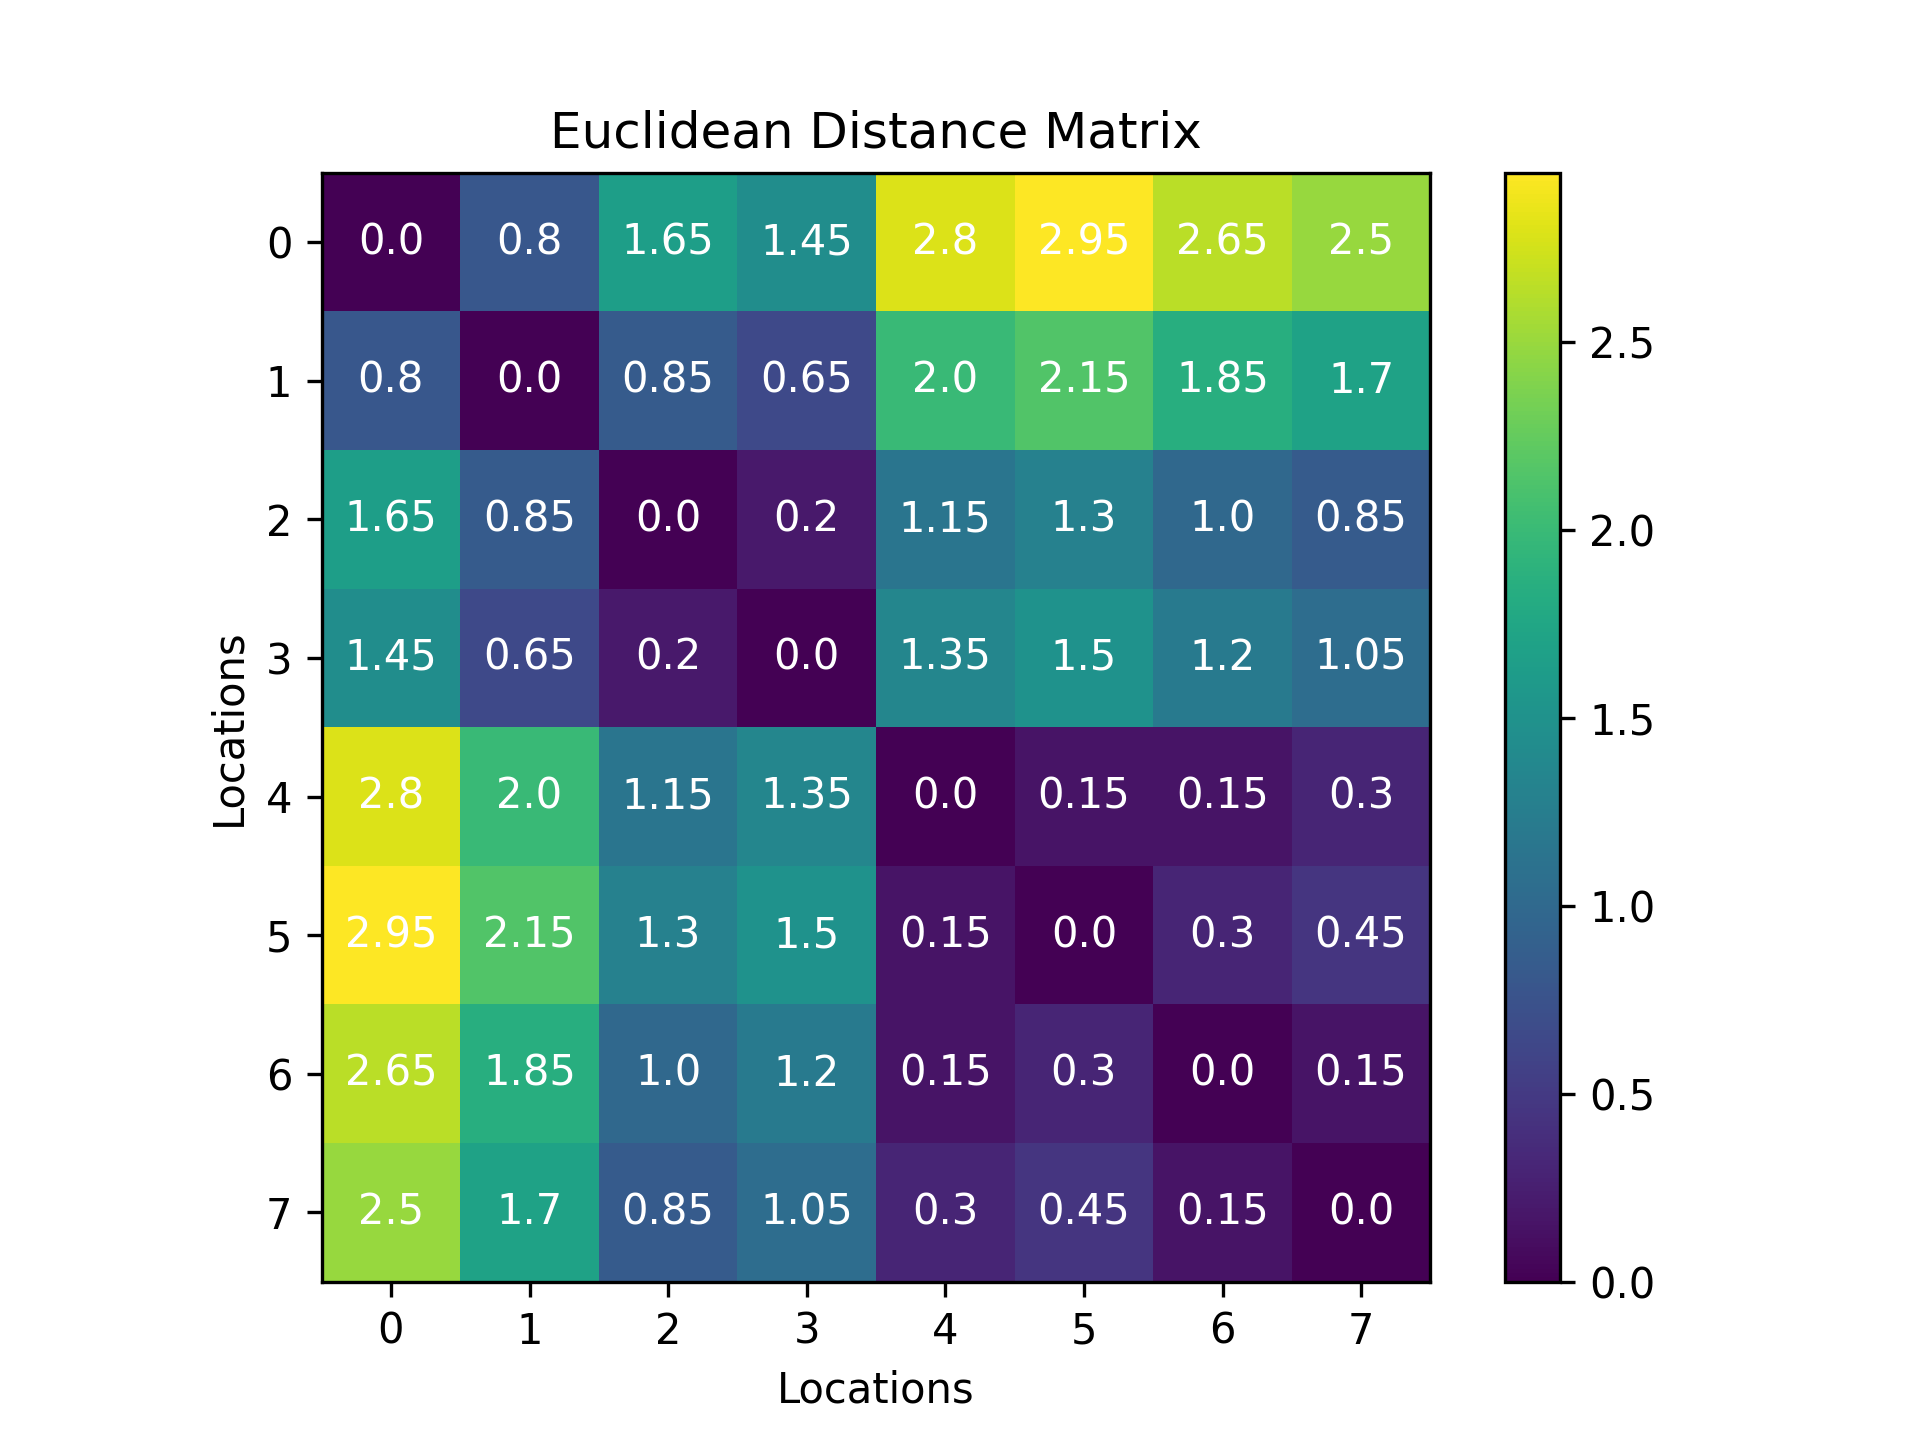
\includegraphics[width=0.9\textwidth]{images/research_design/distance_matrix_lab.png}
        \captionof{figure}{Distance matrix for lab.}
        \label{fig:distance_matrix_lab}
    \end{minipage}%
    \begin{minipage}{0.5\textwidth}
        \centering
        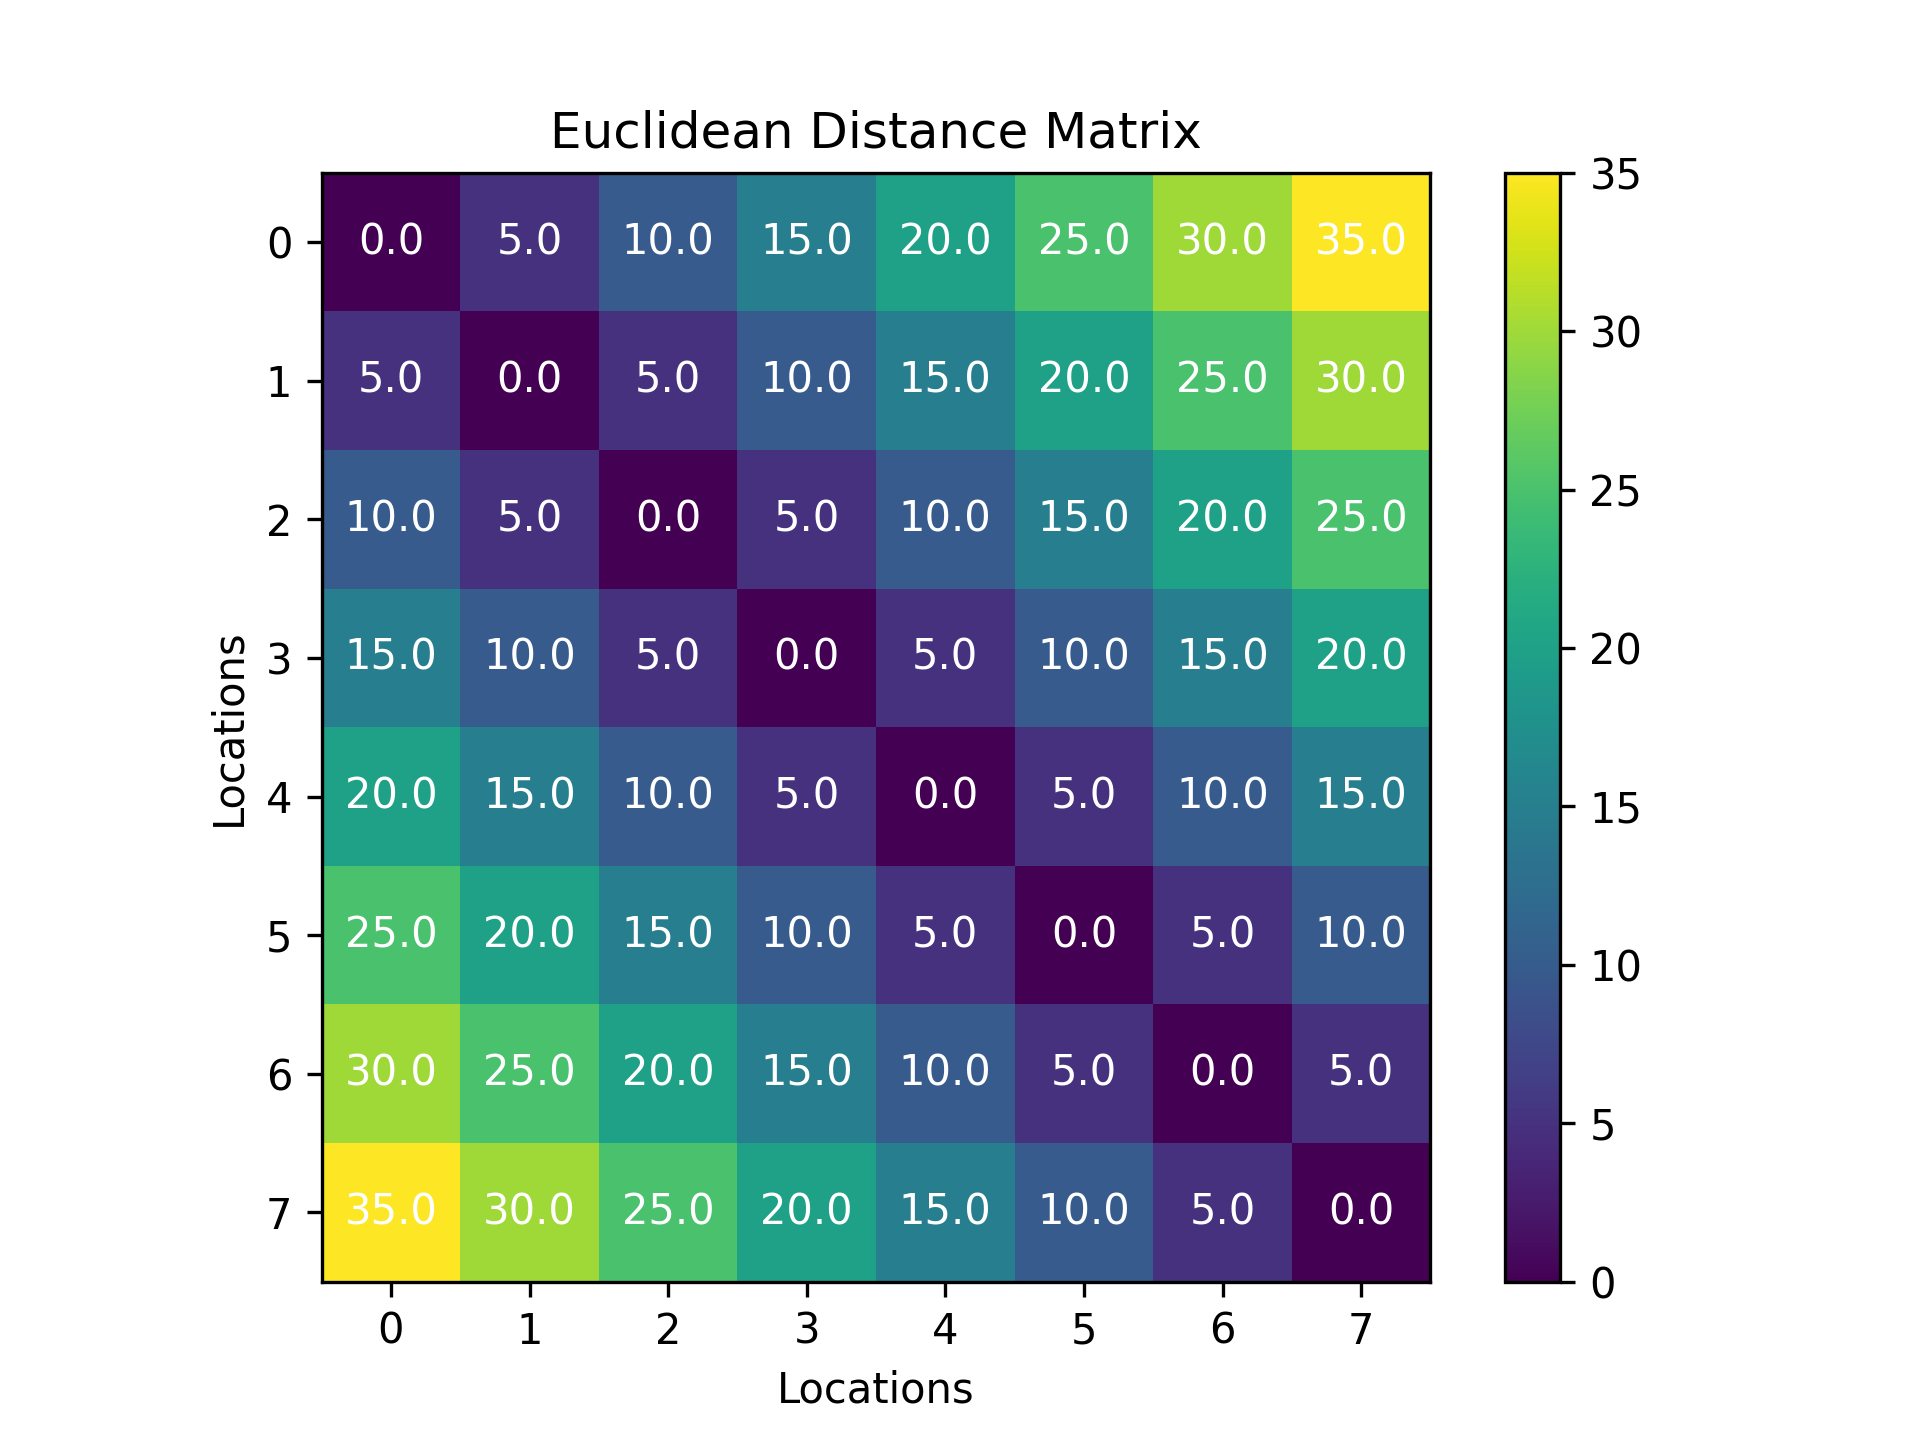
\includegraphics[width=0.9\textwidth]{images/research_design/distance_matrix_home.png}
        \captionof{figure}{Distance matrix for home.}
        \label{fig:distance_matrix_home}
    \end{minipage}
\end{figure}

These distances played a crucial role in our data collection, allowing us to analyze the impact of distance on our system's performance.


\subsection{Data Collection Methodology}\label{sec:data_collection_methodology}
The data collection process utilized various modes, time periods, and data types to analyze system performance, as detailed below:

\vspace{2mm}
\begin{enumerate}
    \item \textbf{Modes: }Two modes were employed: \textit{Maximum} and \textit{Optimized}. Maximum mode operated at $8 dBm$, while Optimized mode used Monte Carlo Method and Genetic Algorithm outputs for transmission power.
    \item \textbf{Time Periods:} 60 $seconds$ was selected for the \textit{Lab} location and 300 $seconds$ for the \textit{Home} location, capturing a larger data set for each location.
    \item \textbf{Data Types:} Data was collected with \textit{No Sensor} connected and with Thread \textit{ICMP Ping}, measuring power consumption under different conditions.
\end{enumerate}
\vspace{3mm}

Data was collected using the nRF Power Profiler Kit II at $100,000$ samples per second. More extended time periods or higher ping rates would have resulted in excessive data, complicating the analysis process.

A table illustrating the data collection process is provided.


% \begin{table}[htbp]
%   \centering
%   \begin{tblr}{
%     colspec={|X[1]|X[1]|X[1]|X[1]|X[1]|X[1]|},
%     hlines, vlines,
%     row{1} = {font=\bfseries},
%   }
%   Location & Mode & Time Period & Data Type & Ping Frequency & Input Voltage \\
%   \SetCell[r=4]{l} Lab & \SetCell[r=2]{l} Maximum & \SetCell[r=4]{l} $60 seconds$ & No Sensor & $0$& \SetCell[r=8]{l} $3.588V$ \\
%   & & & ICMP Ping & $50$ & \\
%   & \SetCell[r=2]{l} Optimized & & No Sensor & $0$ & \\
%   & & & Ping & $50$ & \\
%   \SetCell[r=4]{l} Home & \SetCell[r=2]{l} Maximum & \SetCell[r=4]{l} $300 seconds$ & No Sensor & $0$ & \\
%   & & & ICMP Ping & 290 & \\
%   & \SetCell[r=2]{l} Optimized & & No Sensor & $0$ & \\
%   & & & ICMP Ping & $290$ & \\
%   \end{tblr}
%     \caption{Data collection methodology.}
%     \label{tab:data_collection_methodology}
% \end{table}

\begin{longtblr}[
  caption = {Data collection methodology.},
  label = {tab:data_collection_methodology},
  ]{
  colspec = {|X[1]|X[1]|X[1]|X[1]|X[1]|X[1]|},
  hlines, vlines,
  rowhead = 1, % Repeat the header row on every page
  row{1} = {font=\bfseries},
}
  Location & Mode & Time Period & Data Type & Ping Frequency & Input Voltage \\
  \SetCell[r=4]{l} Lab & \SetCell[r=2]{l} Maximum & \SetCell[r=4]{l} 60 $seconds$ & No Sensor & 0& \SetCell[r=8]{l} 3.588 $V$ \\
  & & & ICMP Ping & 50 & \\
  & \SetCell[r=2]{l} Optimized & & No Sensor & 0 & \\
  & & & Ping & 50 & \\
  \SetCell[r=4]{l} Home & \SetCell[r=2]{l} Maximum & \SetCell[r=4]{l} 300 $seconds$ & No Sensor & 0 & \\
  & & & ICMP Ping & 290 & \\
  & \SetCell[r=2]{l} Optimized & & No Sensor & 0 & \\
  & & & ICMP Ping & 290 & \\
\end{longtblr}

\subsection{Device Setup}\label{sec:device_setup}
This section discusses preparing various device types and modes for data collection.

\subsubsection{Source Meter Mode for Routers and REEDs}\label{sec:source_meter_mode}
For Routers and REEDs, we used the nRF PPK2 in Source Meter mode to measure the current flow and deliver power to the devices. Each device operated at an input voltage of 3.588V. The Source Meter mode allowed us to accurately measure the current flowing through the devices during the data collection.

\begin{figure}[h]
    \centering
    \begin{minipage}[t]{0.45\textwidth}
        \centering
        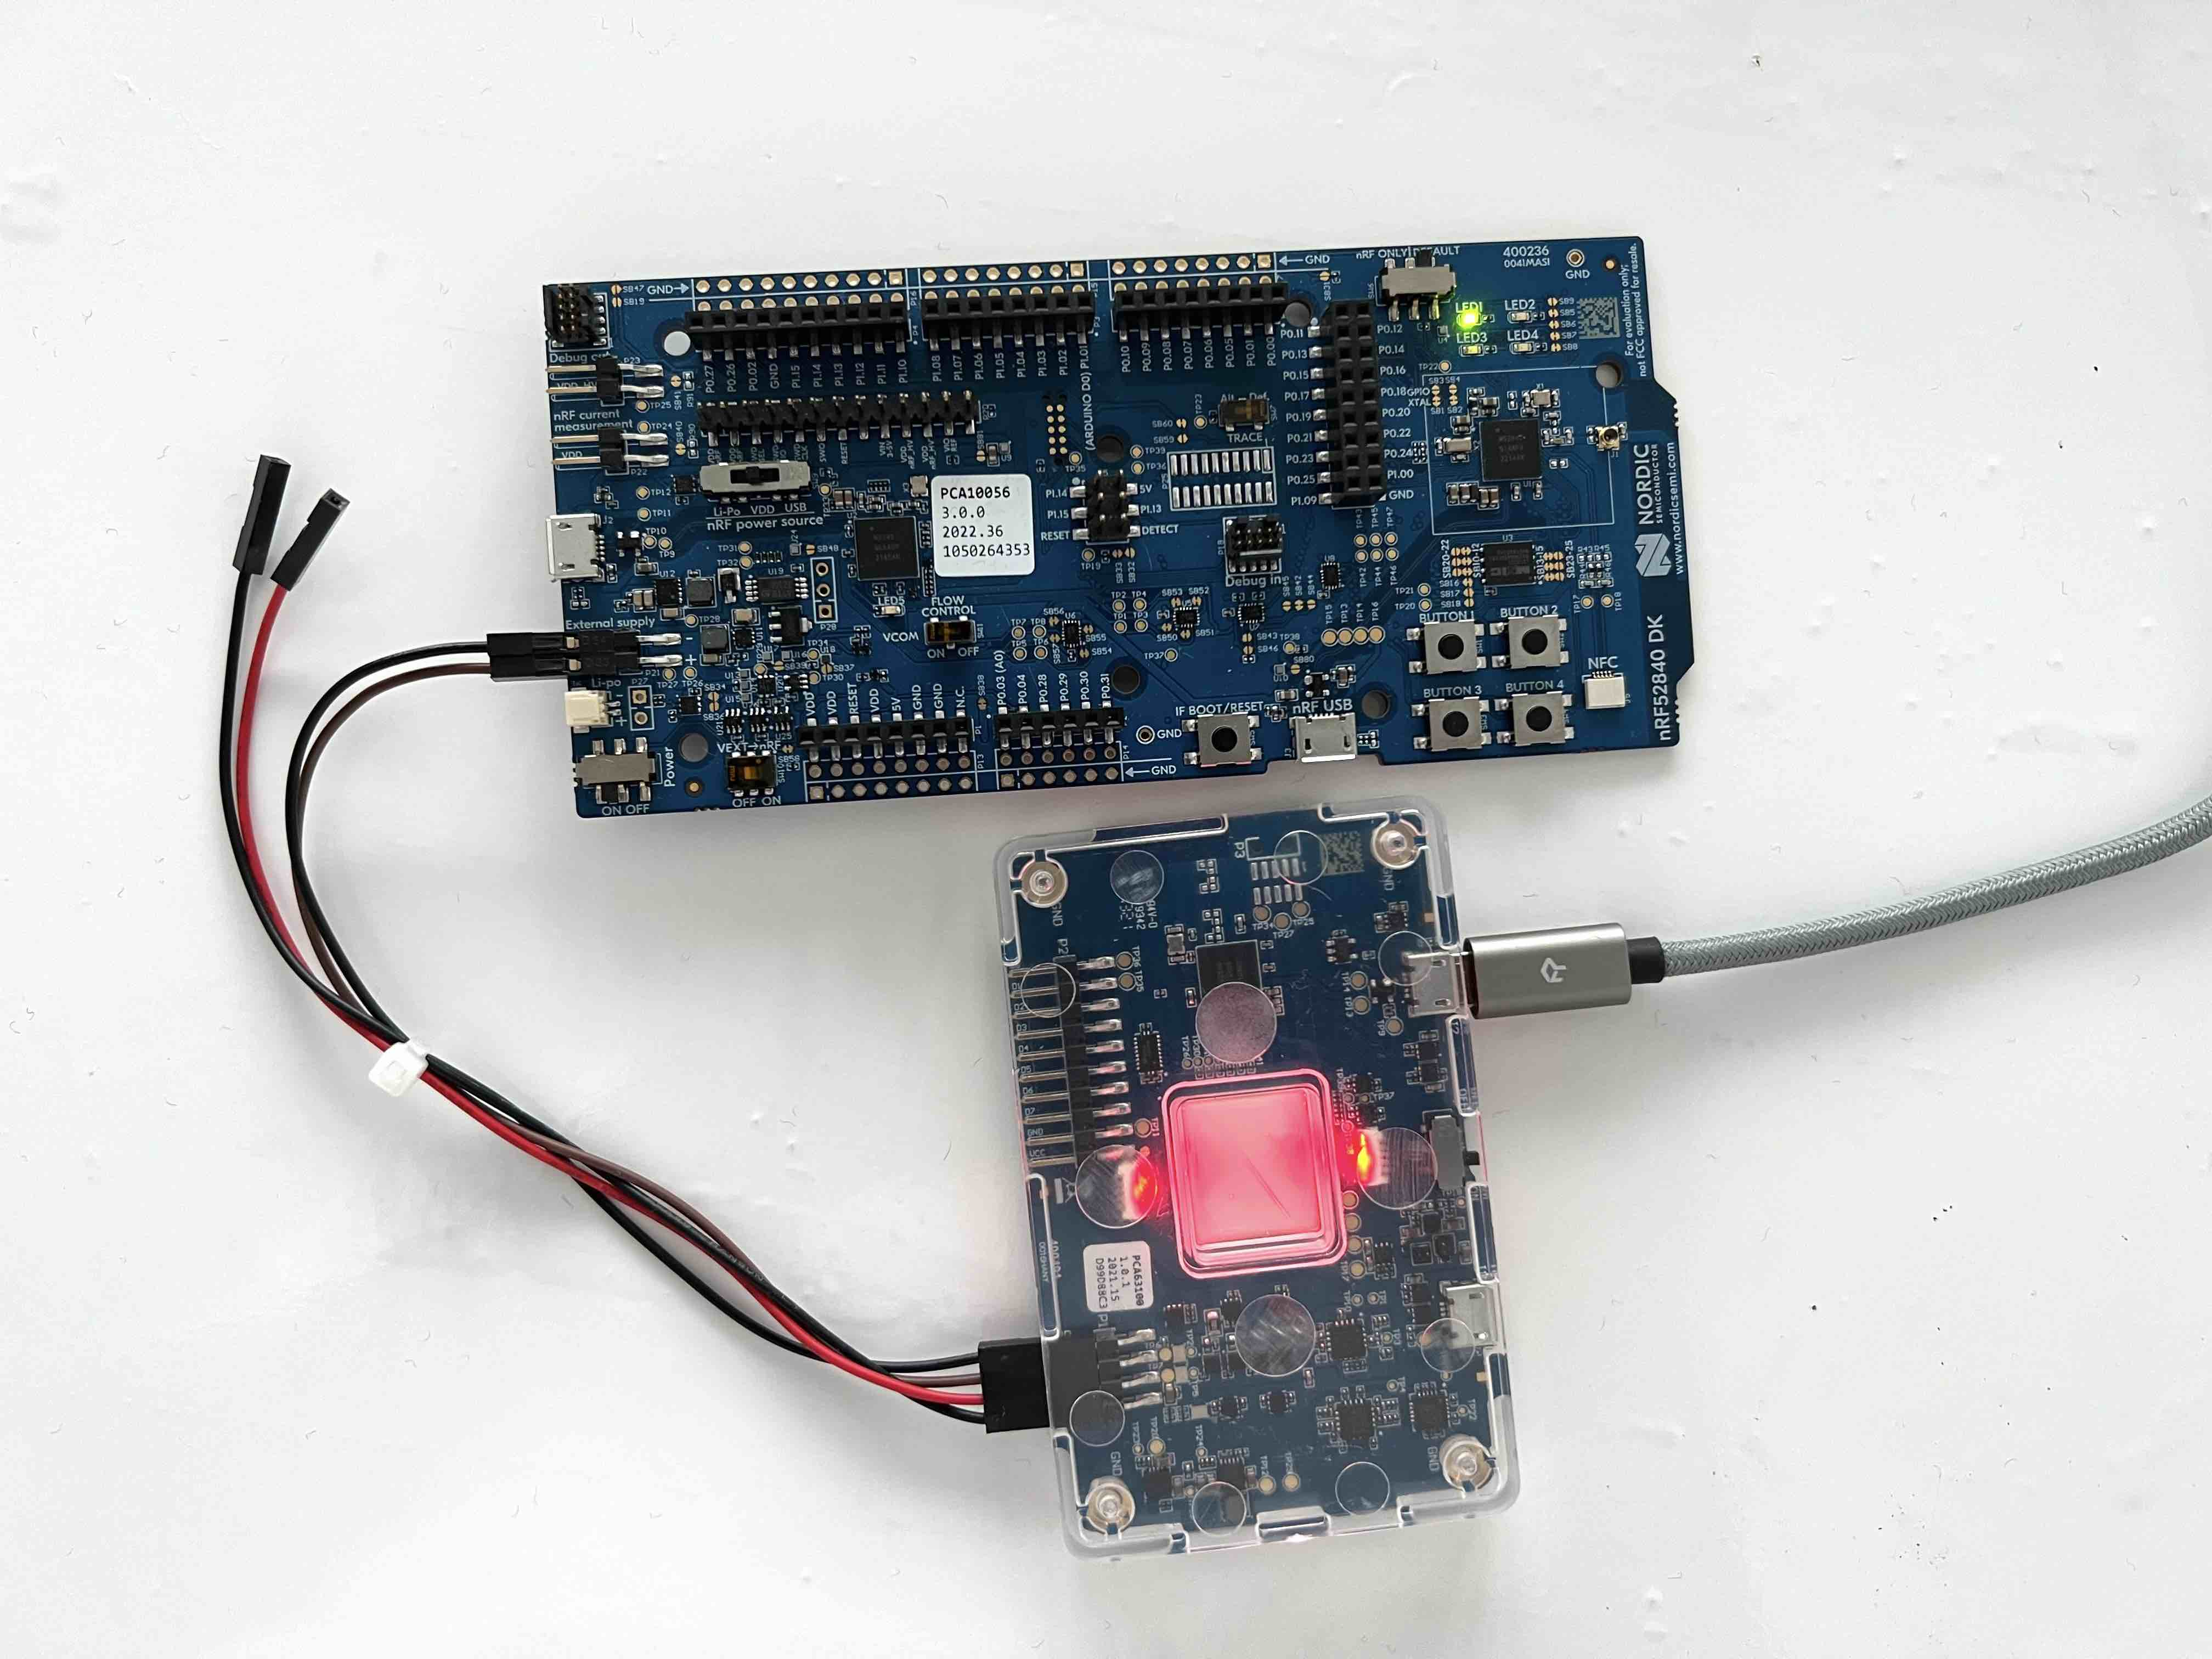
\includegraphics[width=0.7\linewidth]{images/research_design/PPK2_Router.jpg}
        \captionof{figure}{PPK2 connected to a Router.}
        \label{fig:router_source_meter}
    \end{minipage}\hfill
    \begin{minipage}[t]{0.45\textwidth}
        \centering
        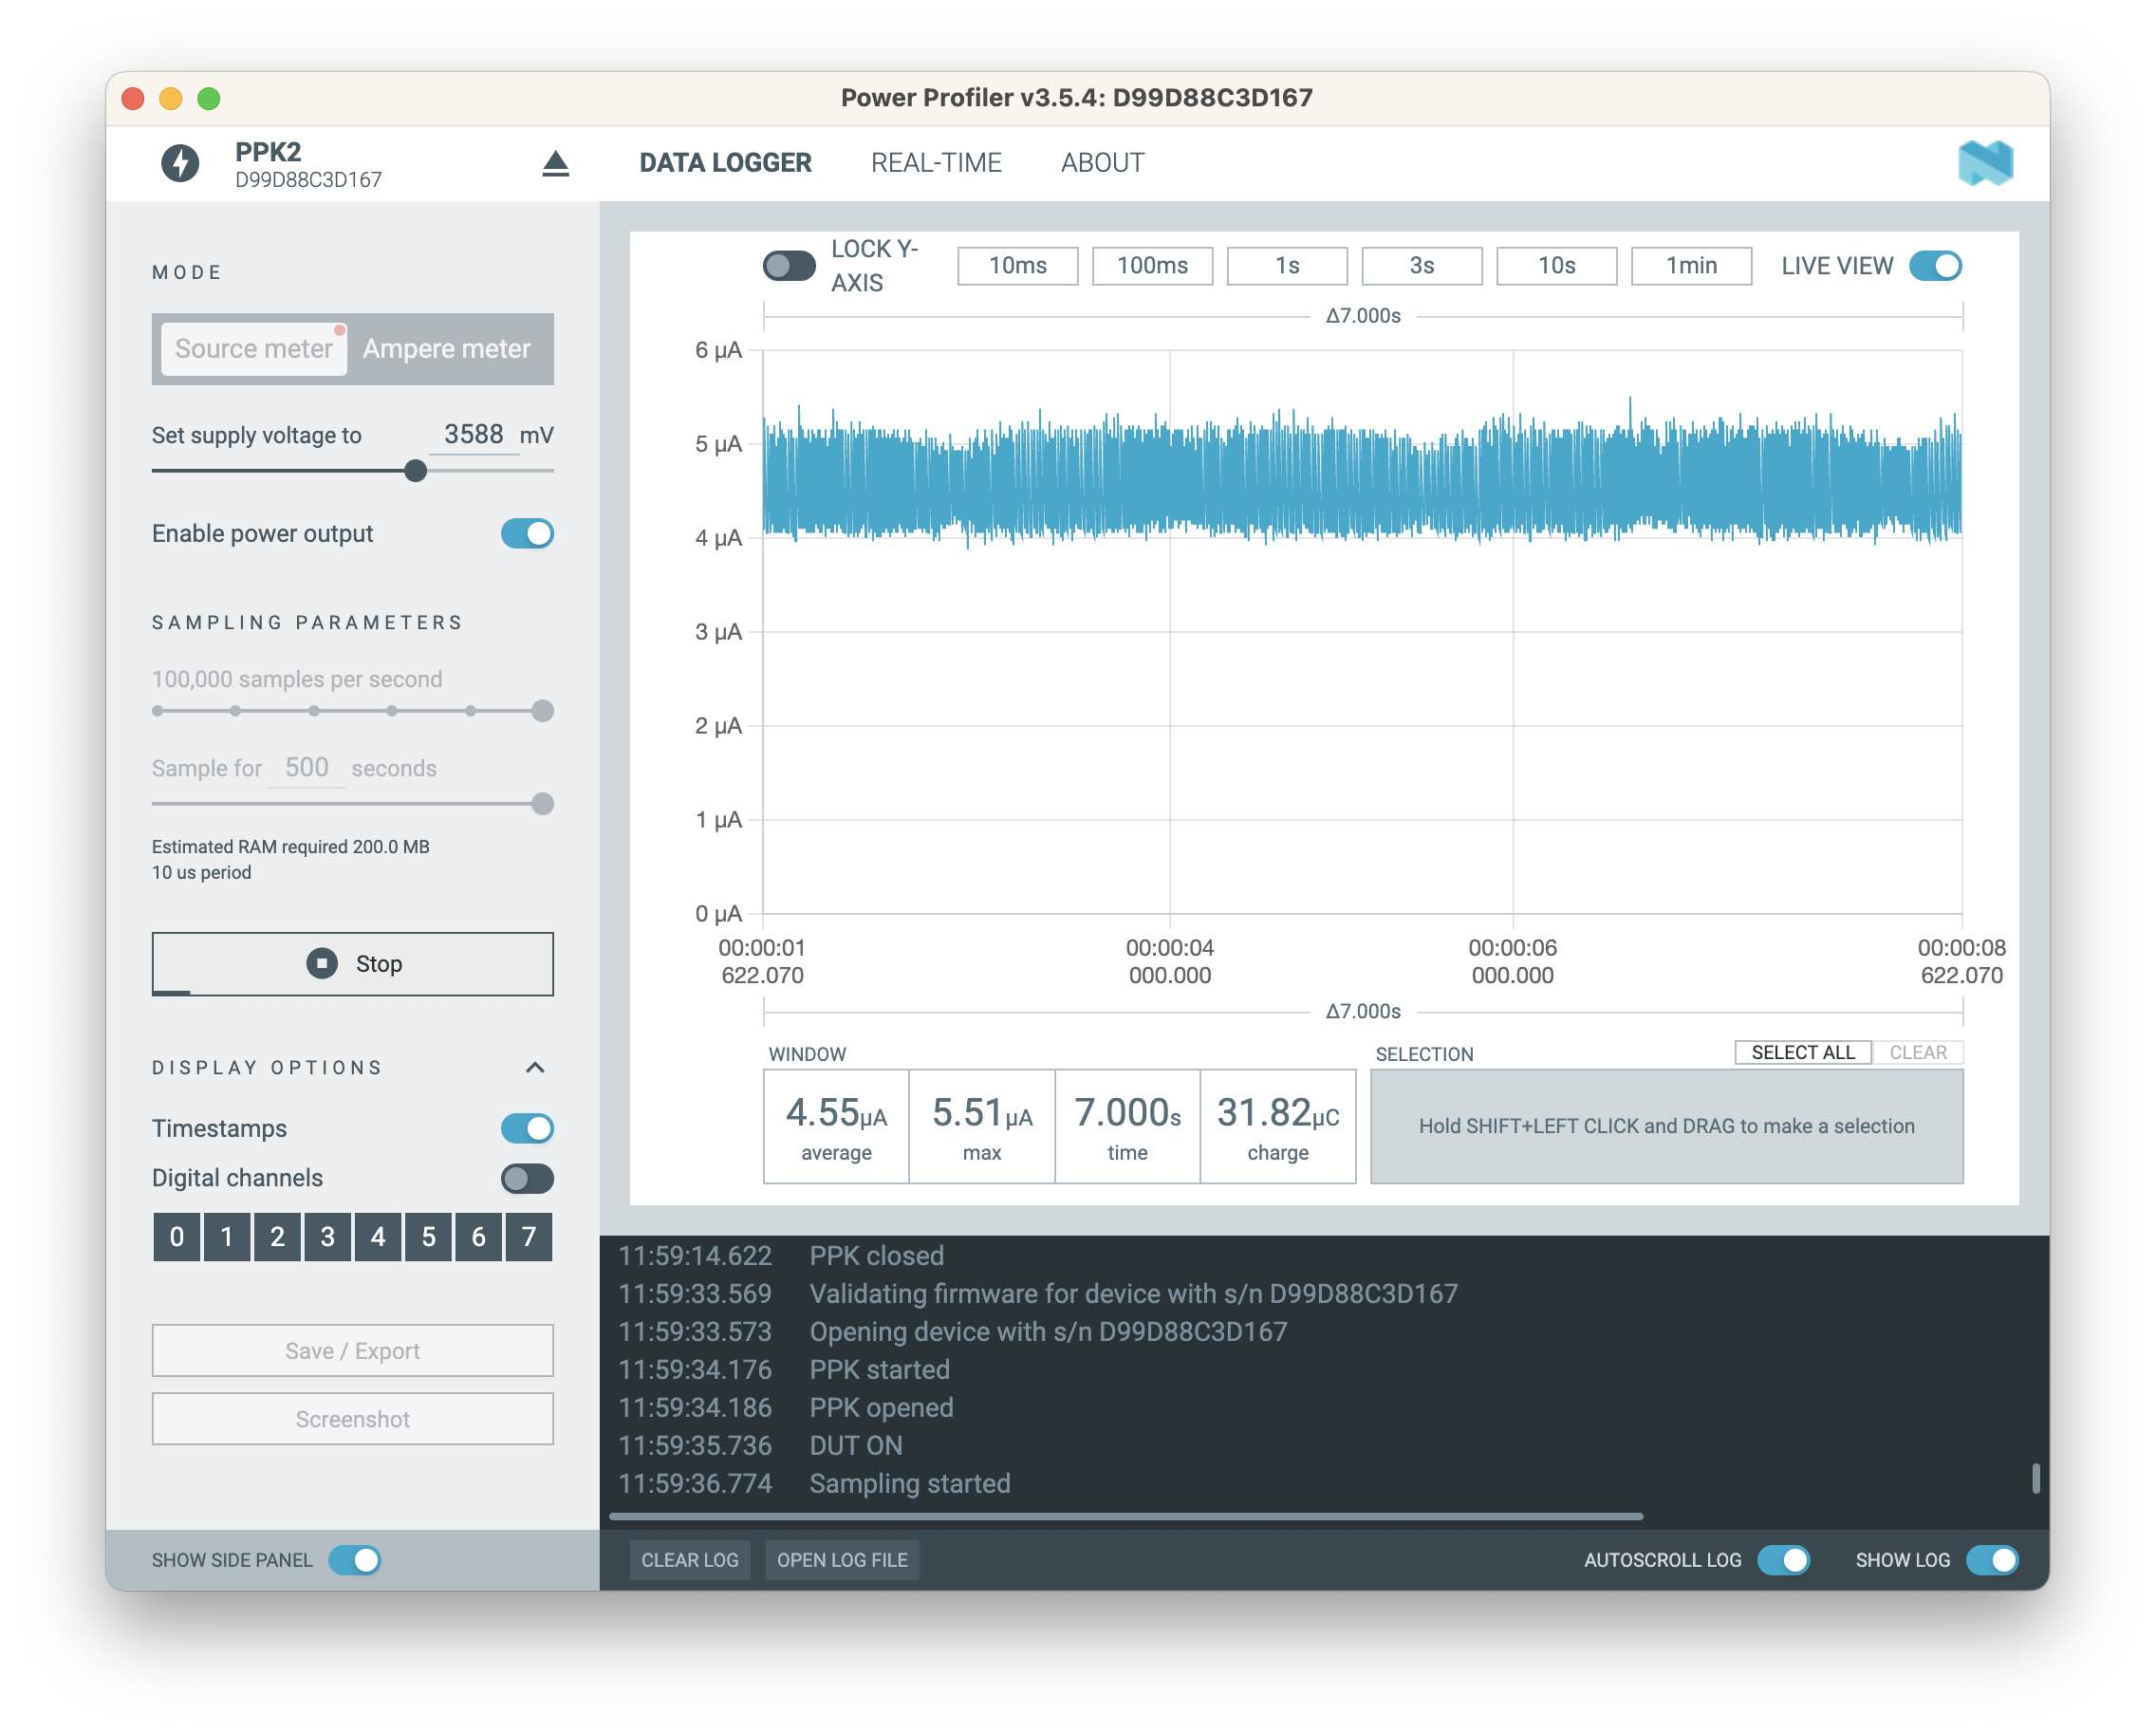
\includegraphics[width=0.7\linewidth]{images/research_design/PPK2_SDK.jpg}
        \captionof{figure}{PPK2 Software in Source Meter mode.}
        \label{fig:ppk2_source_meter}
    \end{minipage}
\end{figure}

Figure \ref{fig:router_source_meter} displays current measurement using the nRF PPK2 from the nRF 52840 DK and Figure \ref{fig:ppk2_source_meter} shows the current measurement in Source Meter mode using the Power Profiler software.

\subsubsection{Ampere Meter Mode for Border Routers}\label{sec:ampere_meter_mode}
Since the USB connection cannot be used with Source Meter mode, and the Border Routers require a connection from the Edge device (Raspberry Pi) to the nRF device to run the RCP (Radio Coprocessor), we used the nRF PPK2 in Ampere Meter mode to measure the current flow for the Border Routers.

\begin{figure}[h]
    \centering
    \begin{minipage}[t]{0.45\textwidth}
        \centering
        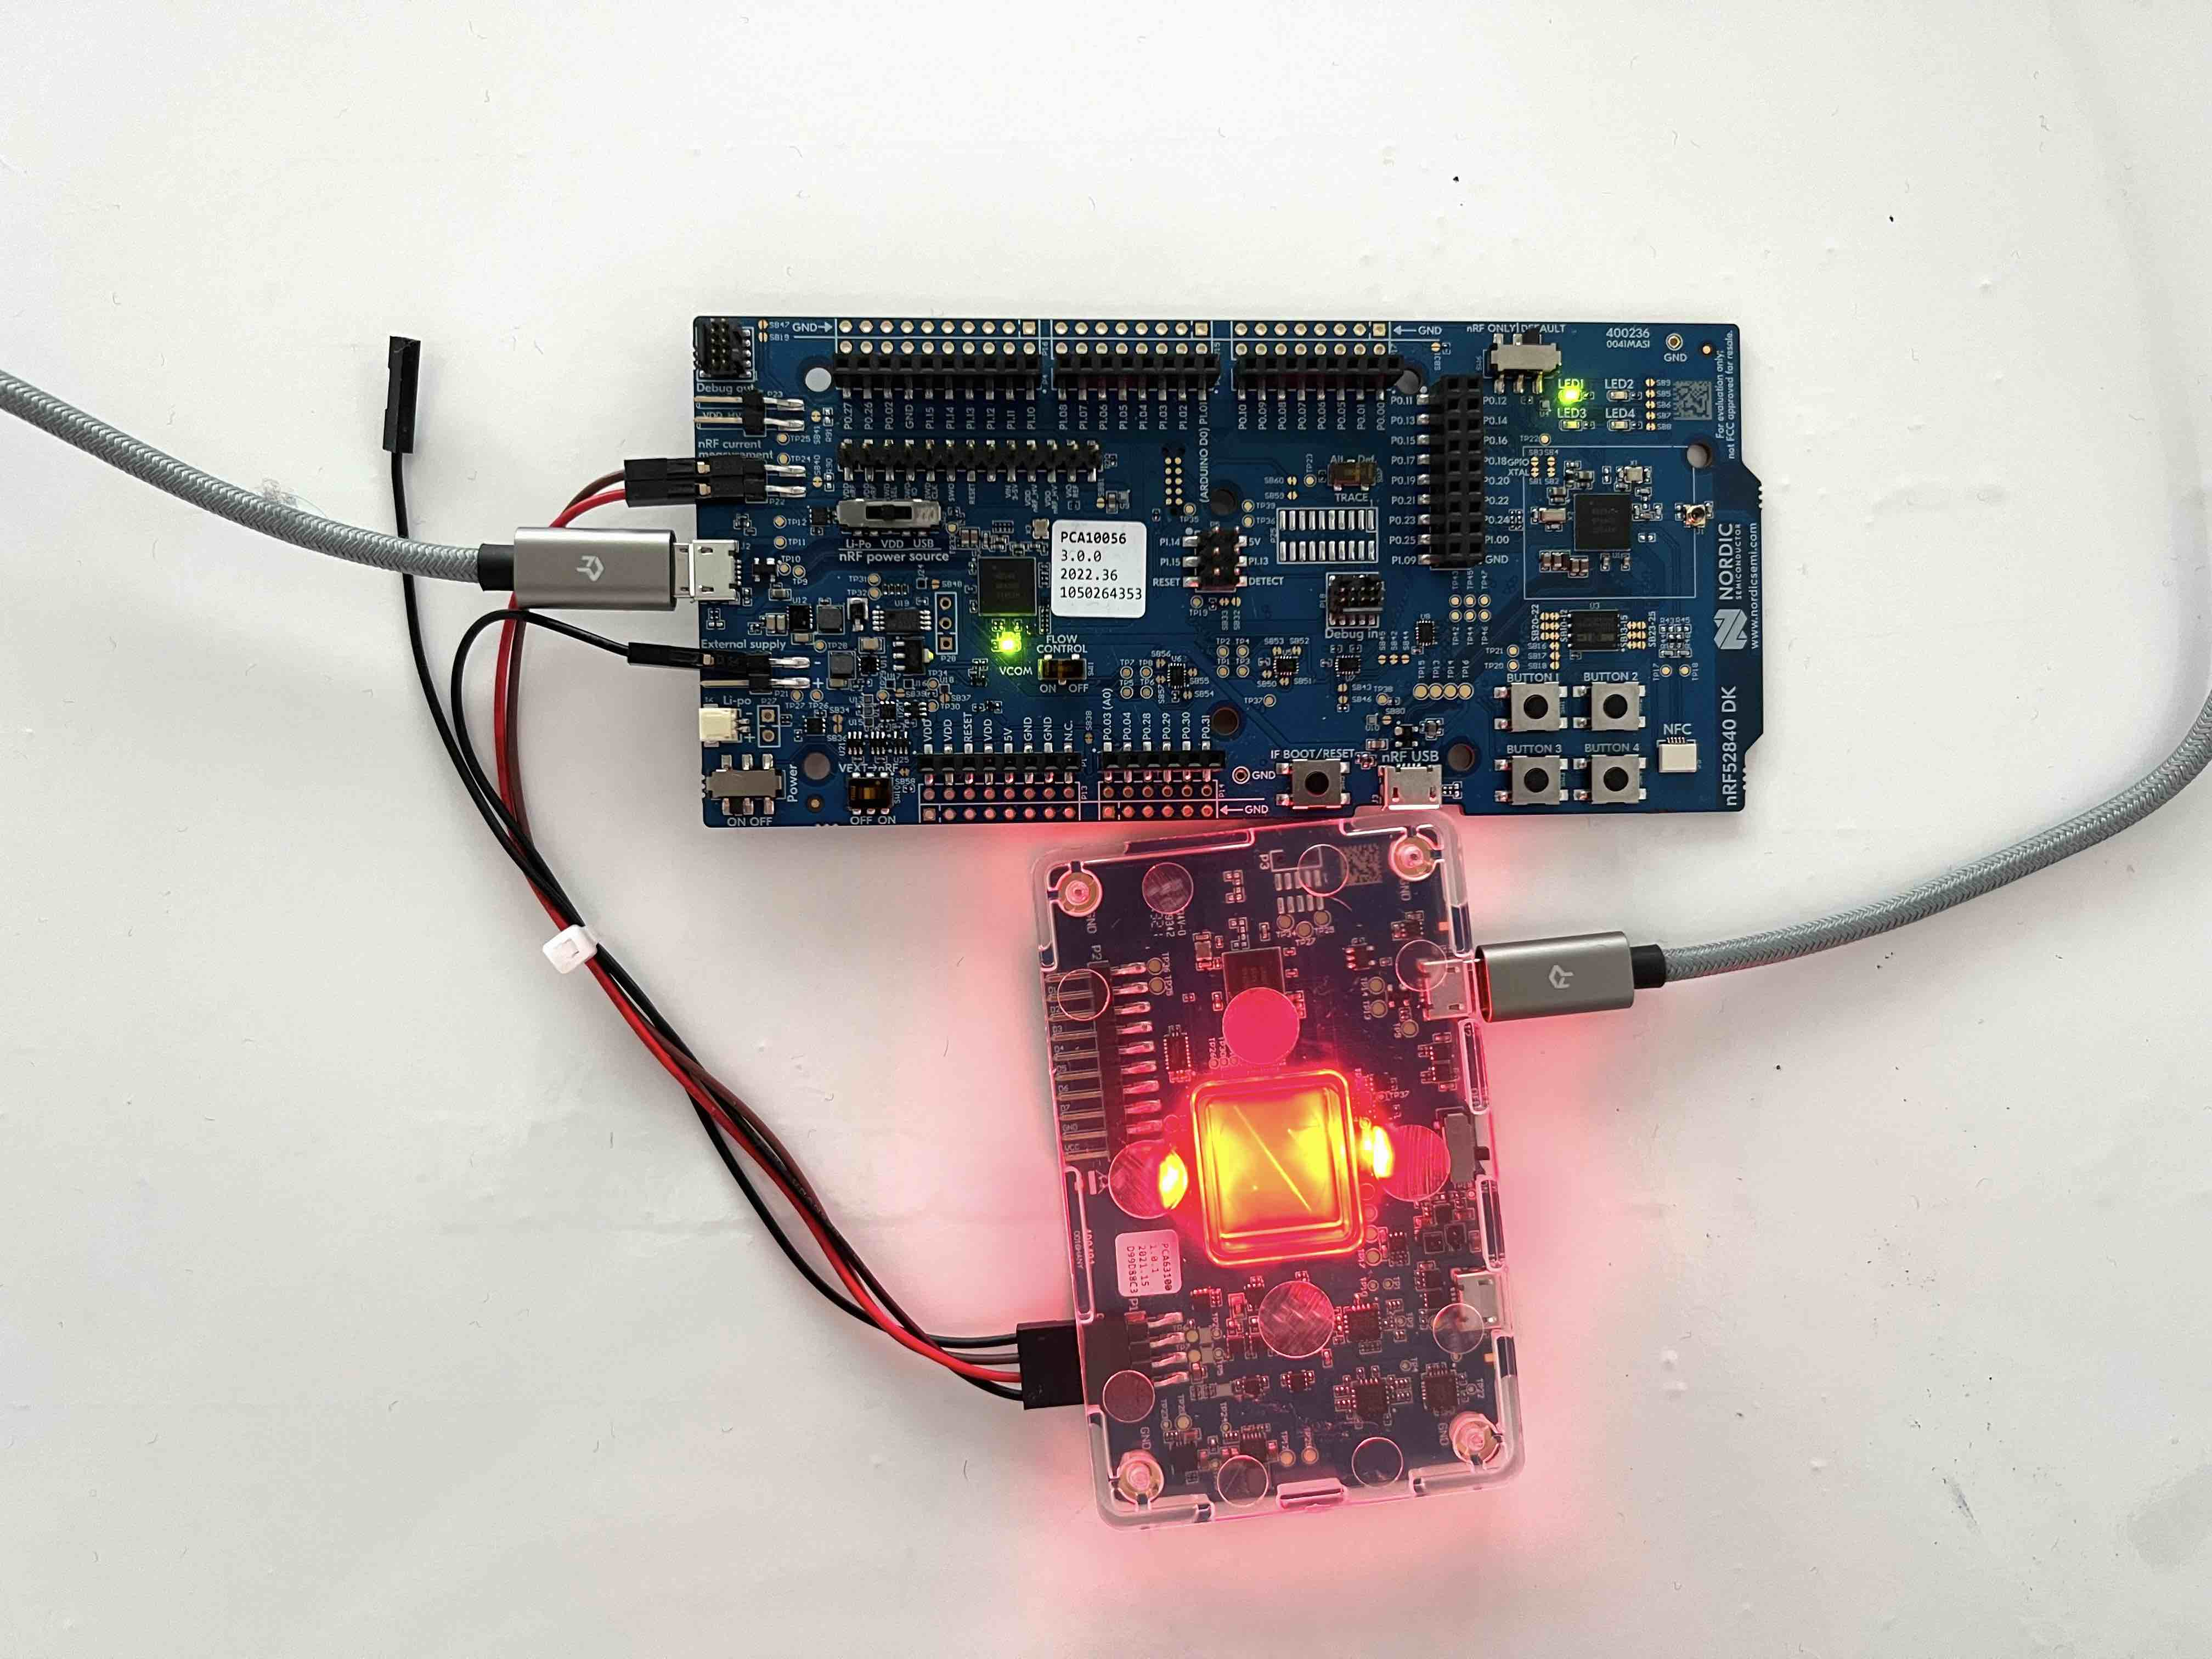
\includegraphics[width=0.7\linewidth]{images/research_design/PPK2_Border_Router.jpg}
        \captionof{figure}{PPK2 connected to a Border Router.}
        \label{fig:border_router_ampere_meter}
    \end{minipage}\hfill
    \begin{minipage}[t]{0.45\textwidth}
        \centering
        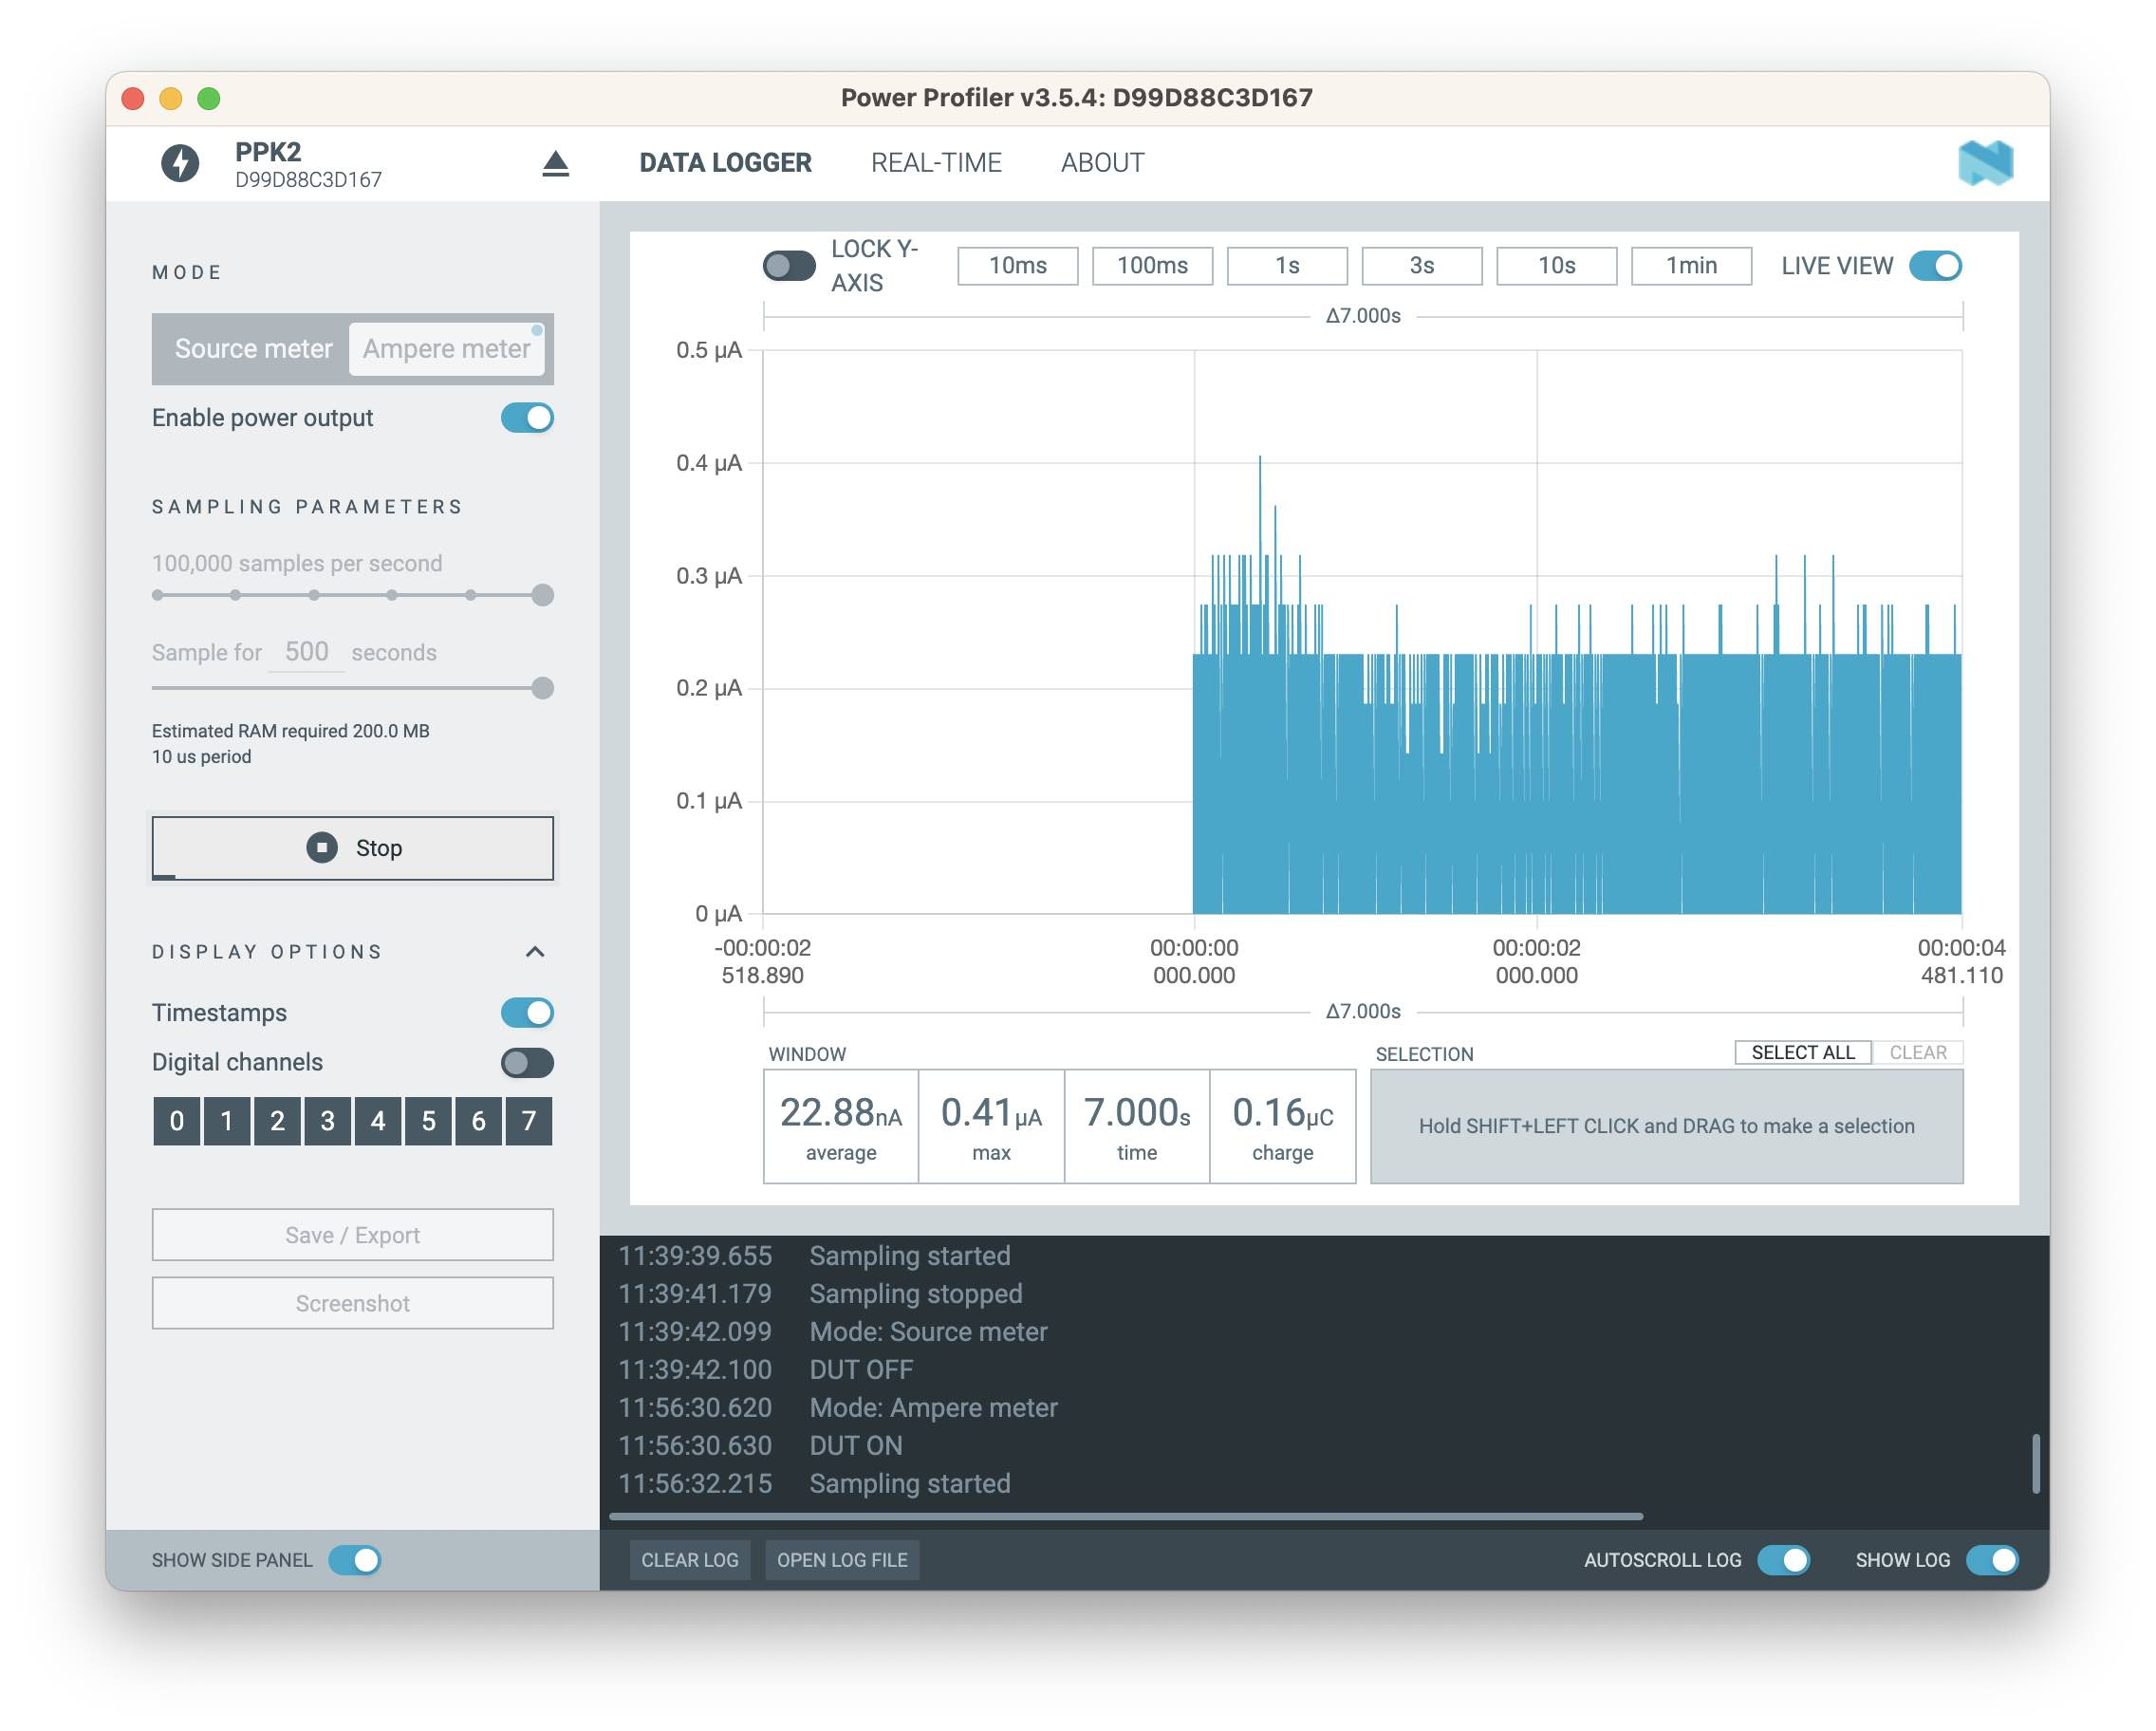
\includegraphics[width=0.7\linewidth]{images/research_design/PPK2_SDK_Ampere.jpg}
        \captionof{figure}{PPK2 Software in Ampere Meter mode.}
        \label{fig:ppk2_ampere_meter}
    \end{minipage}
\end{figure}

Figure \ref{fig:border_router_ampere_meter} displays current measurement using the nRF PPK2 from the nRF 52840 DK and Figure \ref{fig:ppk2_ampere_meter} shows the current measurement in Ampere Meter mode using the Power Profiler software.

\vspace{2mm}
To accurately measure the current from Border Routers during data collection, the SB40 bridge connection from the SoC was cut so that the current flowed through the PPK2 only and not through the USB. This modification enabled precise current flow measurements.

The prototype, built using specific hardware, was optimized using Monte Carlo simulations and Genetic Algorithms for the transmission power of a Thread network. This provided valuable insights into network performance under various conditions and was a basis for further analysis and validation.
